%%%%%%%%%%%%%%%%%%%%%%%%%%%%%%%%%%%%%%%
% Project N°3 for ITY
% Author: Michal Ormos
% Date : 4.4.2015
%%%%%%%%%%%%%%%%%%%%%%%%%%%%%%%%%%%%%%%

\documentclass[a4paper, 11pt]{article}
\usepackage[left=2cm,text={17cm,24cm},top=3cm]{geometry}
\usepackage[czech]{babel}
\usepackage[T1]{fontenc}
\usepackage[utf8]{inputenc}
\usepackage{times}
\usepackage[ruled,czech,linesnumbered,longend,noline]{algorithm2e}
\usepackage{algorithmic}
\usepackage{graphics}
\usepackage{picture}
\usepackage{array}

\begin{document}

%%%% Title Page %%%%
\begin{titlepage}
\begin{center}
\huge
\textsc{\Huge Vysoké učení technické v~Brně
\\\huge Fakulta informačních technologií}

\vspace{\stretch{0.382}}
\Large{Typografie a publikování -- 3. projekt}\\
\Huge{Tabulky a obrázky}
\vspace{\stretch{0.618}}
\end{center}

{\Large 31. března 2015 \hfill Michal Ormoš}
\end{titlepage}
%%%% Title Pa29e %%%%

\newpage
\pagestyle{plain}

\section{Úvodní strana}
Název práce umístěte do zlatého řezu a nezapomeňte uvést dnešní datum a vaše jméno a přijmení.

\section{Tabulky}
Pro sázení tabulek můžeme použít buď prostředí \texttt{tabbing} nebo prostředí \texttt{tabular}.

\subsection{Prostředí \texttt{tabbing}}
Při použití \texttt{tabbing} vypadá tabulka následovně:
\begin{tabbing}

Vodní melouny \quad \= 25,90 \quad \= Množství \= \kill
\textbf{Ovoce}\> \textbf{Cena}\> \textbf{Množství}\\
Jablka \> 25,90 \> 3\,kg\\
Hrušky \> 27,40 \> 2,5\,kg\\
Vodní melouny \> 35,-- \> 1\,kus\\
\end{tabbing}

\noindent Toto prostředí se dá také použít pro sázení algoritmů, ovšem vhodnejší je použít prostředí \texttt{algorithm} nebo \texttt{algorithm2e}  (viz sekce \ref{sec:Algoritmy}).

\subsection{Prostředí \texttt{tabular}}
Další možností jak vytvořit tabulku je použít prostředí \texttt{tabular}. Tabulky pak budou vypadat takto\footnote{Kdyby byl problem s~\texttt{cline}, zkuste se podívat třeba sem: http://www.abclinux.cz/tex/poradna/show/325037.}:
\bigskip
\begin{table}[h]
\begin{center}
\catcode`\-=12
\begin{tabular}{| l | r | r |} \hline
& \multicolumn{2}{|c|}{\textbf{Cena}} \\ \cline{2-3}
\textbf{Měna} & \textbf{nákup} & \textbf{prodej} \\ \hline
EUR & 27,34 & 27,42 \\
JPY & 33,09 & 33,21 \\
USD & 19,87 & 19,95 \\ \hline
\end{tabular}
\caption{Tabulka kurzů k~dnešnímu dni}
\label{tab:tab1}
\end{center}
\end{table}

\begin{table}[h]
\begin{center}
\catcode`\-=12
  \begin{tabular}{| c | c |} \hline
    $A$ & $\neg A$\\ \hline
    \textbf{P} & N\\ \hline
    \textbf{O} & O\\ \hline
    \textbf{X} & X\\ \hline
    \textbf{N} & P\\ \hline
  \end{tabular}
  \begin{tabular}{| c | c | c | c | c | c |} \hline
    \multicolumn{2}{| c |}{} & \multicolumn{4}{| c |}{$B$}\\ \cline{3-6}
    \multicolumn{2}{| c |}{$A \wedge B$} & \textbf{P} & \textbf{O} & \textbf{X} & \textbf{N}\\ \hline
    & \textbf{P} & P & O~& X & N\\ \cline{2-6}
    & \textbf{O} & O~& O~& N & N\\ \cline{2-6}
    $A$
    & \textbf{X} & X & N & X & N\\ \cline{2-6}
    & \textbf{N} & X & N & X & N\\ \hline
  \end{tabular}
  \begin{tabular}{| c | c | c | c | c | c |} \hline
    \multicolumn{2}{| c |}{} & \multicolumn{4}{| c |}{$B$}\\ \cline{3-6}
    \multicolumn{2}{| c |}{$A \vee B$} & \textbf{P} & \textbf{O} & \textbf{X} & \textbf{N}\\ \hline
    & \textbf{P} & P & P & P & P\\ \cline{2-6}
    & \textbf{O} & P & O~& P & O\\ \cline{2-6}
    $A$
    & \textbf{X} & P & P & X & X\\ \cline{2-6}
    & \textbf{N} & P & O~& X & N\\ \hline
  \end{tabular}
  \begin{tabular}{| c | c | c | c | c | c |} \hline     %VYCENTRUJ KONJUNKCIU DISJKUNKCIU A SIPKU
    \multicolumn{2}{| c |}{} & \multicolumn{4}{| c |}{$B$}\\ \cline{3-6}
    \multicolumn{2}{| c |}{$A \rightarrow B$} & \textbf{P} & \textbf{O} & \textbf{X} & \textbf{N}\\ \hline
    & \textbf{P} & P & O~& X & N\\ \cline{2-6}
    & \textbf{O} & O~& O~& P & O\\ \cline{2-6}
    $A$
    & \textbf{X} & P & P & X & X\\ \cline{2-6}
    & \textbf{N} & P & P & P & P\\ \hline
  \end{tabular}
\caption{Protože Kleeneho trojhodnotová logika je už "zastaralá", uvádíme si zde příklad čtyřhodnotové logiky}
\label{tab:tab2}
\end{center}
\end{table}

\newpage

\section{Algoritmy} \label{sec:Algoritmy}
Pokud budeme chtít vysázet algoritmus, můžeme použít prostředí \texttt{algorithm}\footnote{Pro nápověda, jak zacházet s~prostředím \texttt{algorithm}, můžeme zkusit tuhle stránku: http://ftp.cstug.cz/pub/tex/CTAN/macros/latex/contrib/algorithms/algorithms.pdf.} nebo \texttt{algorithm2e}\footnote{Pro \texttt{algorithm2e} zase tuhle: http://ftp.cstug.cz/pub/tex/CTAN/macros/latex/contrib/algorithm2e/doc/algorithm2e.pdf.} . Příklad použití prostředí \texttt{algorithm2} viz Algoritmus \ref{alg:algoritmus1}.

\bigskip  
\algsetup{indent=2em}
\begin{algorithm}[H]
\caption{\textsc{Fast}SLAM}
\label{alg:algoritmus1}
%\SetKwInOut{Input}{Input}
\SetKwInput{Input}{Input}
\SetKwInOut{Output}{Output}
\SetNlSty{}{}{:  }
\SetInd{1em}{1em}
\SetNlSkip{-1.33em}

\Input{$(X_{t-1},u_t,z_t)$}
\Output{$X_t$}
\BlankLine
\Indp \Indp
    $\overline{X_t} = X_t = 0$\\
    \For{$k=1$ \textnormal{to} $M$}
    { 
    %\Indp
        $x_t^{[k]} =$ \emph{sample\_motion\_model}$(u_t,x_{t-1}^{[k]})$\\
        $w_t^{[k]} =$ \emph{measurement\_model}$(z_t,x_t^{[k]},m_{t-1})$\\
        $m_t^{[k]} = updated\_occupancy\_grid(z_t,x_t^{[k]},m_{t-1}^{[k]})$\\
        $\overline{X_t} = \overline{X_t} + \langle x_x^{[m]},w_t^{[m]}\rangle$
    }
    \For{$k=1$ \textnormal{to} $M$}
    {
        draw $i$ with probability $\approx w_t^{[i]}$\\
        add $\langle x_x^{[k]},m_t^{[k]}\rangle$ to $X_t$\\
    }
    \Return{$X_t$}
\end{algorithm}
\bigskip

\section{Obrázky}
Do našich článků můžeme samozřejme vkládat obrázky. Pokud je obrázkem fotografie, můžeme klidně použít bitmapový soubor. Pokud by to ale mělo být nějaké chéma nebo něco podobného, je dobrým zvykem takovýto obrázek vytvořit vektorově.

\begin{figure}[h]
\begin{center}
  \scalebox{0.4}
  {
    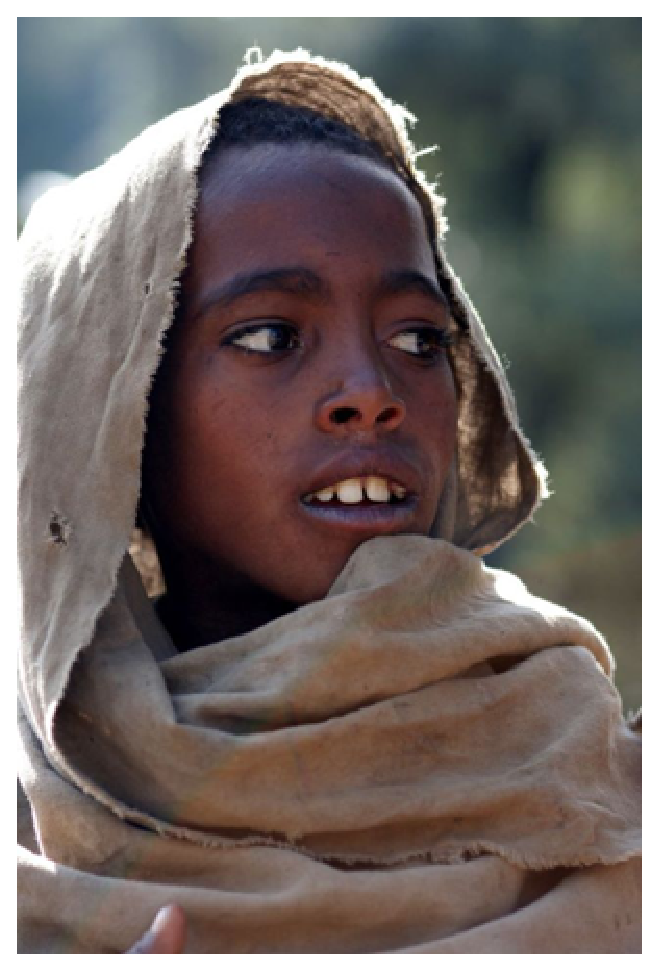
\includegraphics{etiopan.eps}
    \reflectbox{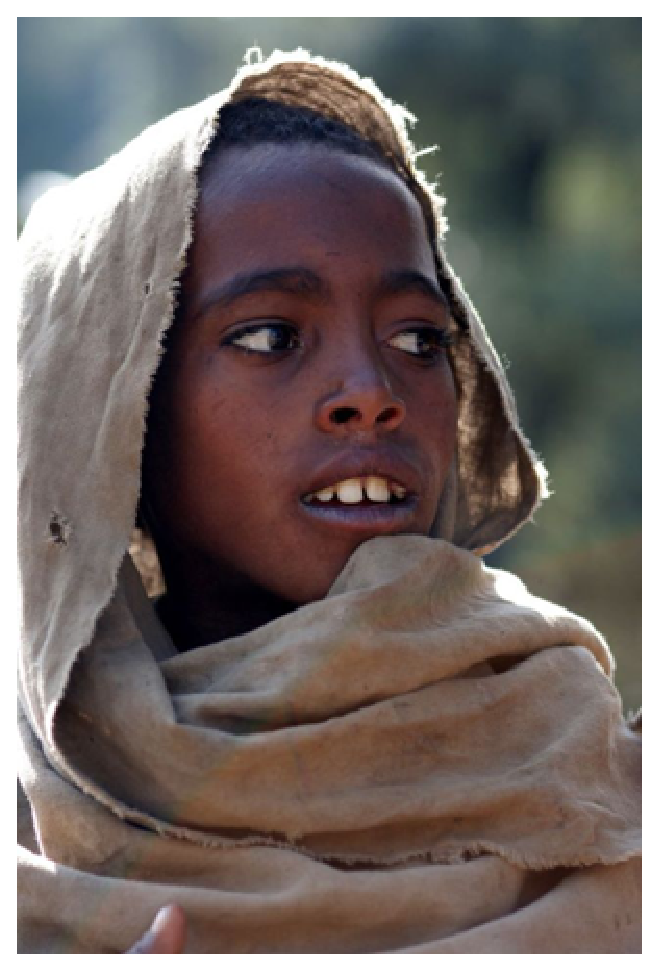
\includegraphics{etiopan.eps}} 
  }
  \caption{Malý Etiopánek a jeho bratříček}
  \label{pic:obr1}
\end{center}
\end{figure}

\newpage

Rozdíl mezi vektorovým\,\ldots
\begin{figure}[h]
\begin{center}
  \scalebox{0.4}
  {
    
\includegraphics{oniisan.eps}
  }
  \caption{Vektorový obrázek}
  \label{pic:obr2}
\end{center}
\end{figure}

\noindent\ldots\,a bitmapovým obrázkem

\begin{figure}[h]
\begin{center}
  \scalebox{0.6}
  {
    
\includegraphics{oniisan2.eps}
  }
  \caption{Bitmapový obrázek}
  \label{pic:obr3}
\end{center}
\end{figure}

 se projeví například při zvětšení


Odkazy (nejen ty) na obrázky \ref{pic:obr1}, \ref{pic:obr2} a \ref{pic:obr3} na tabulky \ref{tab:tab1}, \ref{tab:tab2} a také na algoritmus \ref{alg:algoritmus1} jsou udělány pomocí křížových odkazů. Pak je ovšem potřeba zdrojový soubor přeložit dvakrát.

Vektorové obrázky lze vytvořit i přímo v~\LaTeX u, například pomocí prostředí \texttt{picture}. Všechny rozmeřy jsou uváděny v~mm.

\newpage

\begin{figure}
\begin{center}
\setlength{\unitlength}{1.35mm}
\begin{picture}(115,158.5)
\put(0,0){\linethickness{1pt}\framebox(115,158.5){}}

%pravé vektory a popisky
\put(88,151.25){\vector(0,1){7.25}}
\put(88,151.25){\vector(0,-1){7.25}}
\put(90,144){\makebox(15,14.5){\shortstack{Výška \\ mezery\,=\,14,5}}}
\put(88,139){\vector(0,1){5}}
\put(88,139){\vector(0,-1){5}}
\put(89,132){\makebox(15,14.5){\shortstack{Výška \\ mezery\,=\,10}}}
\put(88,129){\vector(0,1){5}}
\put(88,129){\vector(0,-1){5}}
\put(89,122){\makebox(15,14.5){\shortstack{Výška \\ hlavièky\,=\,10}}}
\put(88,117){\vector(0,1){7}}
\put(88,117){\vector(0,-1){7}}
\put(89,110){\makebox(15,14.5){\shortstack{Výška \\ mezery\,=\,14}}}
\put(88,72.5){\vector(0,1){37.5}}
\put(88,72.5){\vector(0,-1){37.5}}
\put(89,55){\makebox(15,14.5){\shortstack{Výška\\ tìla\,=\,75}}}
\put(88,27.5){\vector(0,1){7.5}}
\put(88,27.5){\vector(0,-1){7.5}}
\put(89,17){\makebox(15,14.5){\shortstack{Výška\\ mezery\,=\,15}}}
\put(88,15){\vector(0,1){5}}
\put(88,15){\vector(0,-1){5}}
\put(89,4){\makebox(15,14.5){\shortstack{Výška\\ paty\,=\,10}}}
%okrajova poznamka
\put(94.5,77){\linethickness{1pt}\framebox(15,10){\textbf{\shortstack{Okrajová\\ poznámka}}}}
\put(88,96.5){\makebox(20,14.5){\shortstack{Mezera\,=\,9}}}
\put(96,102){\vector(-1,-2){6}}
\put(90,90){\vector(-1,0){4.5}}
\put(90,90){\vector(1,0){4.5}}
\put(92,87){\makebox(20,14.5){\shortstack{Šířka\\ boxu\,=\,15}}}
\put(102,90){\vector(-1,0){7.5}}
\put(102,90){\vector(1,0){7.5}}
%vyska stranky
\put(94,43){\makebox(15,14.5){\shortstack{Výška\\ stránky\,=\,158,5}}}
\put(102,55){\vector(1,1){10}}
% pravy bocni vektor
\put(112,79.25){\vector(0,1){79.25}}
\put(112,79.25){\vector(0,-1){79.25}}
%dolni vektor a popis
\put(57.5,3){\vector(1,0){57.5}}
\put(57.5,3){\vector(-1,0){57.5}}
\put(52,3){\makebox(10,5){\shortstack{Šířka stránky = 115}}}
%carkovane cary
\multiput(15,151.5)(0,-10){16}{\line(0,1){7}}
\multiput(0,144)(10,0){11}{\line(1,0){7}}
%levy okraj
\put(7.5,90){\vector(1,0){7.5}}
\put(7.5,90){\vector(-1,0){7.5}}
\put(2.5,90){\makebox(10,5){\shortstack{Mezera = 15}}}
%hlavicka
\put(58,137){\vector(1,0){27.5}}
\put(58,137){\vector(-1,0){27.5}}
\put(55,137){\makebox(10,5){\shortstack{Šířka boxu = 55}}}
\put(30.5,124){\linethickness{1pt}\framebox(55,10){\textbf{Hlavička}}}
%telo
\put(30.5,35){\linethickness{1pt}\framebox(55,75){\textbf{Textové tělo}}}
%pata
\put(30.5,10){\linethickness{1pt}\framebox(55,10){\textbf{Pata}}}
\end{picture}
\caption{Vektorový obrázek v~prostředí \texttt{picture}}
\end{center}
\end{figure}

\end{document}
